\chapter{Measures}

Ideally we would like to a have a function $\mu$ that assigns each $E \subset \bfR$ to a number $\mu(E) \in [0,\infty]$. Such a function $\mu$ should possess the following properties:
    \begin{enumerate}[label = \arabic*.,itemsep=1pt,topsep=3pt]
        \item The unit interval should have a measure equal to one \textemdash that is, $\mu \left( [0,1)\right) =1 $;
        \item If $E$ and $F$ are congruent subsets of $\bfR$ then $\mu(E) = \mu(F)$;
        \item If $E_1,E_2,...$ are pairwise disjoint, then $\mu \left( \bigcup_{j = 1}^\infty E_j \right) = \sum_{j = 1}^\infty \mu(E_j)$.
    \end{enumerate}
Unfortunately, a function possessing all of these traits does not exist. 
    \begin{theorem}
        A function $\mu:\cP(\bfR) \rightarrow [0,\infty]$ satisfying (1), (2), and (3) from above does not exist.
    \end{theorem}
        \begin{proof}
            Suppose such a function $\mu$ does exist. By (1) we have $\mu([0,1)) = 1$. Define a relation on $[0,1)$ as follows: $x \sim y$ if and only if $x-y \in \bfQ$. This is an equivalence relation. Using the Axiom of Choice, let $N$ be a set which contains exactly one element from each equivalence class. Now for each $q \in \bfQ \cap [0,1)$, define:
                \begin{equation*}
                \begin{split}
                    N_q = \{x + q \mid N \cap [0,1-q)\} \cup \{x + (q-1) \mid x \in N \cap [1-q,1)\}.
                \end{split}
                \end{equation*}
            That is, the points in $N_q$ are obtained by "rotating" the points in $N$ by a rational number $q$. Clearly $N_q \subset [0,1)$, hence $\bigcup_{q \in \bfQ \cap [0,1)}N_q \subset [0,1)$. 
            We have the following three properties:
                \begin{enumerate}[label = (\alph*),itemsep=1pt,topsep=3pt]
                    \item For any $q \in \bfQ$, $\mu(N) = \mu(N_q)$
                    \item If $r,s \in \bfQ$, $r \neq s$, then $N_r \cap N_s = \emptyset$.
                    \item For every $y \in [0,1)$, there exists a $q \in \bfQ$ such that $y \in N_q$.
                \end{enumerate}
            Property (a) follows from the fact that $N$ and $N_r$ are congruent, hence:
                \begin{equation*}
                \begin{split}
                    \mu(N) 
                    & = \mu \bigl( N \cap [0,1-q) \bigr) + \mu\bigl(N \cap [1-q,1)\bigr) \\
                    & = \mu\bigl( \{x + q \mid x \in N \cap [0,1-q)\}\bigr) + \mu \bigl( \{x + q - 1 \mid x\in N \cap [1-q,1)\}\bigr) \h9\text{\tiny "Rotation"} \\
                    & = \mu(N_r).
                \end{split}
                \end{equation*}
            Property (b) follows by contradiction \textemdash if $x \in N_r \cap N_s$, then $x - r$ and $x - s$ would be distinct elements of $N$. However, $(x-r) - (x-s) = s-r \in \bfQ$, so $x-r$ and $x-s$ are in the same equivalence class. But this contradicts the way which we've constructed $N$. For property (c), given $y \in [0,1)$, let $x \in \N$ satisfy $x \sim y$. Since $x$ and $y$ are in the same equivalence class, we can find $q \in \bfQ$ such that:
                \begin{equation*}
                \begin{split}
                    y =
                    \begin{cases}
                        x+q, & x < y \\
                        x - (q-1) & x > y
                    \end{cases}.
                \end{split}
                \end{equation*}
            Hence $y \in N_q$, giving $[0,1) \subset N_q \subset \bigcup_{q \in \bfQ \cap [0,1)}N_q$. We've obtained the equality:
                \begin{equation*}
                \begin{split}
                    \bigcup_{q \in \bfQ \cap [0,1)}N_q = [0,1).
                \end{split}
                \end{equation*}
            Property (b) says that this is a disjoint union:
                \begin{equation*}
                \begin{split}
                    \bigsqcup_{q \in \bfQ \cap [0,1)}N_q = [0,1).
                \end{split}
                \end{equation*}
            Finally, with property (a), we have:
                \begin{equation*}
                \begin{split}
                    1
                    & = \mu([0,1)) \\
                    & = \mu \left( \bigsqcup_{q \in \bfQ \cap [0,1)}N_q \right) \\
                    & = \sum_{q \in \bfQ \cap [0,1)}\mu(N_q) \\
                    & = \sum_{n = 1}^\infty \mu(N).
                \end{split}
                \end{equation*}
            This is impossible, hence there does not exist a $\mu$ satisfying (1), (2), and (3).
        \end{proof}

    A good guess for this failure would be that we assumed countable additivity as opposed to finite additivity. This is not the case. In dimensions $n \geq 3$, assuming such a weak form of $\mu$ leads to the following result:
        \begin{theorem}[Banach-Tarski]
            Let $U$ and $V$ be arbitrary bounded open sets in $\bfR^n$ for $n \geq 3$. There exist $k \in \bfN$ and subsets $E_1,...,E_k$, $F_1,...,F_k$ of $\bfR^n$ such that:
                \begin{itemize}
                    \item the $E_j$'s are disjoint and their union is $U$;
                    \item the $F_j$'s are disjoint and their union is $V$;
                    \item $E_j$ is congruent to $F_j$ for all $1 \leq j \leq k$.
                \end{itemize}
        \end{theorem}
    Ultimately, the problem comes from the fact we defined $\mu$ on \textit{every possible} subset of $\bfR$. We can't hope to do this, since as we showed there exists bizarre sets like $N$ which cannot be measured. Instead, we will define $\mu$ on a special class of subsets of $\bfR^n$.

\section{$\sigma$-Algebras}
    \begin{definition}
        Let $X$ be a set. An \textit{algebra of sets} $\cA \subset \cP(X)$ is a collection of subsets of $X$ which is:
            \begin{enumerate}[label = (\arabic*),itemsep=1pt,topsep=3pt]
                \item closed under finite union: if $E_1,E_2,...,E_n \in \cA$, then $\bigcup_{i = 1}^n E_n \in \cA$;
                \item closed under complement: if $E \in \cA$, then $E^c \in \cA$.
            \end{enumerate}
        If $\cA$ is closed under countable union, then we say $\cA$ is a \textit{$\sigma$-algebra}.
    \end{definition}

    \begin{proposition}
        Let $\cA$ be an algebra of sets.
        \begin{enumerate}[label = (\arabic*),itemsep=1pt,topsep=3pt]
            \item $\cA$ is closed under finite intersection.
            \item $\cA$ is closed under set difference.
            \item $\emptyset \in \cA$ and $X \in \cA$.
        \end{enumerate}
    \end{proposition}
        \begin{proof}
            (1) Let $E_1,E_2,...,E_n \in \cA$. Then $\bigcap_{i = 1}^n E_i = \left( \bigcup_{i=1}^n E_i^c \right)^c \in \cA$. (2) If $E_1,E_2 \in \cA$, then $E_1 \setminus E_2 = E_1 \cap E_2^c \in \cA$. (3) For any $E \in \cA$, we have $\emptyset = E \cap E^c \in \cA$ and $X = E \cup E^c \in \cA$.
        \end{proof}

    \begin{proposition}
        Let $\cA$ be an algebra of sets. The following are equivalent:
            \begin{enumerate}[label = (\arabic*),itemsep=1pt,topsep=3pt]
                \item $\cA$ is a $\sigma$-algebra.
                \item $\cA$ is closed under countable disjoint union.
            \end{enumerate}
    \end{proposition}
        \begin{proof}
            If $\cA$ is a $\sigma$-algebra, then it is closed under countable union, hence it must be closed under countable disjoint union. Conversely, suppose $\cA$ is closed under countable disjoint union. Let $\{E_n\}_{n = 1}^\infty$ be a family of sets in $\cA$. Define:
                \begin{equation*}
                \begin{split}
                    F_1 &= E_1, \\
                    F_2 &= E_2 \setminus E_1 \\
                    F_3 &= E_3 \setminus (E_1 \cup E_2) \\
                    &\vdots \\
                    F_n &= E_n \setminus \left( E_1 \cup E_2 \cup ... \cup E_{n-1} \right).
                \end{split}
                \end{equation*}
            Let $i < j$ be natural numbers and consider $F_i \cap F_j$. If $x \in F_i$, then $x \in E_i$. Since $i < j$, we have $x \in E_1 \cup ... \cup E_{j-1}$, hence $x \not\in F_j$. Thus $F_i \cap F_j = \emptyset$. Inductively, $\{F_n\}_{n = 1}^\infty$ is a countable family of disjoint sets.

            Clearly $\bigcup_{n = 1}^\infty F_n \subset \bigcup_{n = 1}^\infty E_n$. Conversely, let $x \in \bigcup_{n = 1}^\infty E_n$. Find the smallest natural number $j$ such that $x \in E_j$. Then $x \not\in E_i$ for $i < j$. Hence $x \in E_j \setminus (E_1 \cup ... \cup E_{j-1}) = F_j \subset \bigcup_{n=1}^\infty F_n$.

            Since $\cA$ is closed under countable disjoint unions, we have $\bigcup_{n = 1}^\infty E_n = \bigcup_{n = 1}^\infty F_n \in \cA$. Since $\{E_n\}_{n = 1}^\infty$ was an arbitrary family of sets, this means $\cA$ is a $\sigma$-algebra.
        \end{proof}

    \begin{proposition}
        If $\{\cE_i\}_{i \in I}$ is a family of $\sigma$-algebras, then $\bigcap_{i \in I}\cE_i$ is a $\sigma$-algebra.
    \end{proposition}
        \begin{proof}
            Let $\{E_n\}_{n = 1}^\infty$ be a family of sets contained in $\bigcap_{i \in I}\cE_i$. Then each $\{E_n\}_{n = 1}^\infty$ is contained in $\cE_i$. Since $\cE_i$ is a $\sigma$-algebra for every $i \in I$, we have $\bigcup_{n = 1}^\infty E_n \in \cE_i$ for every $i \in I$, which means $\bigcup_{n = 1}^\infty E_n \in \bigcap_{i \in I}\cE_i$.

            Similarly, let $F \in \bigcap_{i \in I}\cE_i$. Then $F \in \cE_i$ for every $i \in I$. Since $\cE_i$ is a $\sigma$-algebra for every $i \in I$, we have $F^c \in \cE_i$ for every $i \in I$, which means $F^c \in \bigcap_{i \in I}\cE_i$. Thus $\bigcap_{i \in I}\cE_i$ is a $\sigma$-algebra.
        \end{proof}

    \begin{definition}
        Let $X$ be a set and $\cE \subset \cP(X)$. The \textit{$\sigma$-algebra generated by $\cE$} is $\fM(\cE) := \bigcap \{\cA \mid \cE \subset \cA, \cA \h1\text{is a $\sigma$-algebra}\h1\}$.
    \end{definition}

    \begin{lemma}
        If $\cE \subset \fM(\cF)$, then $\fM(\cE) \subset \fM(\cF)$.
    \end{lemma}
        \begin{proof}
            Since $\fM(\cF)$ is a $\sigma$-algebra containing $\cE$, it must contain $\fM(\cE)$, as $\fM(\cE)$ is the smallest $\sigma$-algebra generated by $\cE$.
        \end{proof}

    Given a metric space $X$, we might only be interested in what is generated by its open sets.

    \begin{definition}
        Let $X$ be a metric space and $\tau_X$ the set containing all of its open sets. The \textit{Borel $\sigma$-algebra on $X$} is the set $\cB_X := \fM(\tau_X)$. Members of $\cB_X$ are called \textit{Borel sets}.
    \end{definition}

    {\color{red} Talk about G delta and F sigma sets}.

    \begin{proposition}\label{prop:generators-of-borel}
    $\cB_\bfR$ is generated by each of the following:
        \begin{enumerate}[label = (\arabic*),itemsep=1pt,topsep=3pt]
            \item the open intervals: $\cE_1 = \{(a,b) \mid a < b\}$,
            \item the closed intervals: $\cE_2 = \{[a,b] \mid a < b\}$,
            \item the half-open intervals: $\cE_3 = \{(a,b] \mid a < b\}$ or $\cE_4 = \{[a,b) \mid a < b\}$,
            \item the open rays: $\cE_5 = \{(a,\infty) \mid a \in \bfR\}$ or $\cE_6 = \{(-\infty,a) \mid a \in \bfR\}$,
            \item the closed rays: $\cE_7 = \{(a,\infty) \mid a \in \bfR\}$ or $\cE_8 = \{(-\infty,a) \mid a \in \bfR\}$.
        \end{enumerate}
    \end{proposition}
        \begin{proof}
            We are required to show for each $\cE_i$ that $\fM(\cE_i) = \cB_\bfR$.

            (1) Let $I \in \cE_1$ be an open interval. Then $I \in \cB_\bfR$ because $I$ is an open subset of $\bfR$. From this we have $\cE_1 \subset \cB_\bfR$, but because $\cB_\bfR$ is a $\sigma$-algebra containing $\cE_1$, and $\fM(\cE_1)$ is the smallest $\sigma$-algebra containing $\cE_1$, we have $\fM(\cE_1) \subset \cB_\bfR$. Conversely, let $U \in \tau_\bfR$. Then $U$ is at most the countable union of disjoint open intervals, hence $U \in \fM(\cE_1)$. From this we have $\tau_\bfR \subset \fM(\cE_1)$, but because $\fM(\cE_1)$ is a $\sigma$-algebra containing $\tau_\bfR$, and $\fM(\tau_\bfR)$ is the smallest $\sigma$-algebra containing $\tau_\bfR$, we have $\fM(\tau_\bfR) = \cB_\bfR \subset \fM(\cE_1)$.

            (2) Let $I \in \cE_1$ be an open interval. Then $I^c$ is a closed interval, hence it is contained in $\fM(\cE_2)$. Whence $\fM(\cE_1) \subset \fM(\cE_2)$. Conversely, let $C \in \cE_2$ be a closed interval. Then $C$ can be written as the countable intersection of open sets. This means $C \in \fM(\cE_1)$. Whence $\fM(\cE_2) \subset \fM(\cE_1)$. Thus $\fM(\cE_2) = \fM(\cE_1) = \cB_\bfR$.
            ...
        \end{proof}

    Given two sets $X_1$ and $X_2$ with respective $\sigma$-algebras $\cM_1$ and $\cM_2$, we'd like to better understand what a $\sigma$-algebra on $X_1 \times X_2$ looks like. 

    \begin{definition}
        Let $\{X_\alpha\}_{\alpha \in I}$ be an indexed family of nonempty sets, $X = \prod_{\alpha \in I}X_\alpha$, and $\pi_\alpha:X \rightarrow X_\alpha$ the projection maps. If $\cM_\alpha$ is a $\sigma$-algebra on $X_\alpha$ for each $\alpha$, the \textit{product $\sigma$-algebra} on $X$ is:
            \begin{equation*}
            \begin{split}
                \bigotimes_{\alpha \in I}\cM_\alpha := \fM \Bigl(\{\pi_\alpha^{-1}(E_\alpha) \mid E_\alpha \in \cM_\alpha, \h2 \alpha \in I\}\Bigr)
            \end{split}
            \end{equation*}
    \end{definition}

    The significance of this definition will become clear later. If $X_1$ and $X_2$ are sets with $\sigma$-algebras $\cM_1$ and $\cM_2$ respectively, one might wager a more intuitive definition for the $\sigma$-algebra on $X_1 \times X_2$ to be:
        \begin{equation*}
        \begin{split}
            \fM \Bigl(\{E_1 \times E_2 \mid E_1 \in \cM_1,\h2 E_2 \in \cM_2\}\Bigr).
        \end{split}
        \end{equation*} 
    In fact, these two definitions are equivalent if we're only taking the cartesian product of countably many sets! Before proving this, note that if $E_i \subset X_i$ and $\pi_i:X_1 \times X_2 \rightarrow X_i$ for $i=1,2$, then:
        \begin{equation*}
        \begin{split}
            \pi_1^{-1}(E_1) &= E_1 \times X_2,\\
            \pi_2^{-1}(E_2) &= X_1 \times E_2.
        \end{split}
        \end{equation*}
    We can see that:
        \begin{equation*}
        \begin{split}
            \pi_1^{-1}(E_1) \cap \pi_2^{-1}(E_2)
            & = (E_1 \times X_2) \cap (X_1 \times E_2) \\
            & = \{(e_1,x_2) \mid e_1 \in E_1, x_2 \in X_2 \} \cap \{(x_1,e_2) \mid x_1 \in X_1, e_2 \in E_2\} \\
            & = \{(x,y) \mid (x \in E_1\land x \in X_1) \h2\land\h2 (y \in X_2 \land y \in E_2)\} \\
            & = \{(x,y) \mid x E_1 \land y \in E_2 \} \\
            & = E_1 \times E_2.
        \end{split}
        \end{equation*}

    \begin{proposition}
        Let $A$ be a countable indexing set, $\{X_\alpha\}_{\alpha \in A}$ an indexed family of nonempty sets, $X = \prod_{\alpha \in A}X_\alpha$, $\pi_\alpha:X \rightarrow X_\alpha$ the projection maps, and $\cM_\alpha$ a $\sigma$-algebra on $X_\alpha$ for each $\alpha \in A$. Then $\bigotimes_{\alpha \in A}\cM_\alpha$ is generated by:
            \begin{equation*}
            \begin{split}
                \left\{ \prod_{\alpha \in A}E_\alpha \mid E_\alpha \in \cM_\alpha \right\}
            \end{split}
            \end{equation*}
    \end{proposition}
        \begin{proof}
            Denote $\cO$ as the $\sigma$-algebra generated by $\left\{ \prod_{\alpha \in A}E_\alpha \mid E_\alpha \in \cM_\alpha \right\}$.
            If $E_\alpha \in \cM_\alpha$, then $\pi_\alpha^{-1}(E_\alpha) = \prod_{\beta \in A}E_\beta$, where $E_\beta = X_\beta$ for $\beta \neq \alpha$. This gives the inclusion:
                \begin{equation*}
                \begin{split}
                    \{\pi_\alpha^{-1}(E_\alpha) \mid E_\alpha \in \cM_\alpha, \h2 \alpha \in I\} \subset \cO.
                \end{split}
                \end{equation*}
            But since $\bigotimes_{\alpha \in A}\cM_\alpha$ is the smallest $\sigma$-algebra generated by $\{\pi_\alpha^{-1}(E_\alpha) \mid E_\alpha \in \cM_\alpha, \h2 \alpha \in I\}$, we get: 
                \begin{equation*}
                \begin{split}
                    \bigotimes_{\alpha \in A}\cM_\alpha \subset \cO.
                \end{split}
                \end{equation*}
            Conversely, note that $\prod_{\alpha \in A}E_\alpha = \bigcap_{\alpha \in A}\pi_\alpha^{-1}(E_\alpha)$. Since each $\pi_\alpha^{-1}(E_\alpha)$ is in $\bigotimes_{\alpha \in A}\cM_\alpha$, and since $\bigotimes_{\alpha \in A}\cM_\alpha$ is closed under countable intersections, we have that $\prod_{\alpha \in A}E_\alpha \in \bigotimes_{\alpha \in A}\cM_\alpha$. Hence we have the following inclusion:
                \begin{equation*}
                \begin{split}
                    \left\{ \prod_{\alpha \in A}E_\alpha \mid E_\alpha \in \cM_\alpha \right\} \subset \bigotimes_{\alpha \in A}\cM_\alpha.
                \end{split}
                \end{equation*}
            But since $\cO$ is the smallest $\sigma$-algebra generated by $\left\{ \prod_{\alpha \in A}E_\alpha \mid E_\alpha \in \cM_\alpha \right\}$, it must be the case that $\cO \subset \bigotimes_{\alpha \in A}\cM_\alpha$. Since we showed inclusion in both directions, $\cO = \bigotimes_{\alpha \in A}\cM_\alpha$; i.e., $\bigotimes_{\alpha \in A}\cM_\alpha$ is generated by $\left\{ \prod_{\alpha \in A}E_\alpha \mid E_\alpha \in \cM_\alpha \right\}$.
        \end{proof}

    If there exists a set $\cE_\alpha$ such that $\cM_\alpha = \fM(\cE_\alpha)$, then we can generate the product similar algebra in a different way.

    \begin{lemma}***
        Let $\{X_\alpha\}_{\alpha \in A}$ be a family of nonempty sets, $\cE_\alpha \subset \cP(X_\alpha)$, and $\cM_\alpha := \fM(\cE_\alpha)$ for each $\alpha \in A$. Then $\bigotimes_{\alpha \in A}\cM_\alpha$ is generated by:
            \begin{equation*}
            \begin{split}
                \cF_1 = \{\pi_\alpha^{-1}(E_\alpha) \mid E_\alpha \in \cE_\alpha, \alpha \in A\}.
            \end{split}
            \end{equation*}
        If $A$ is countable and $X_\alpha \in \cE_\alpha$ for each $\alpha$, then $\bigotimes_{\alpha \in A}\cM_\alpha$ is generated by:
            \begin{equation*}
            \begin{split}
                \cF_2 = \left\{\prod_{\alpha \in A}E_\alpha \mid E_\alpha \in \cE_\alpha\right\}.
            \end{split}
            \end{equation*}
    \end{lemma}
        \begin{proof}
            Automatically we have $\cF_1 \subset \bigotimes_{\alpha \in A}\cM$, hence $\fM(\cF_1) \subset \bigotimes_{\alpha \in A}\cM_\alpha$. Conversely, consider the set $S:=\{E \subset X_\alpha \mid \pi_\alpha^{-1}(E) \in \fM(\cF_1)\}$. This set is a $\sigma$-algebra. Indeed, if $\{E_n\}_{n \in \bfN}$ is a family of elements of $S$, then $\{\pi_\alpha^{-1}(E_n)\}_{n \in \bfN}$ is a family of elements of $\fM(\cF_1)$. Since $\fM(\cF_1)$ is a $\sigma$-algebra, we get:
                \begin{equation*}
                \begin{split}
                    \bigcup_{n \in \bfN}\pi_\alpha^{-1}(E_n)
                    & = \pi_\alpha^{-1} \left( \bigcup_{n \in \bfN}E_n \right).
                \end{split}
                \end{equation*}
            Hence $\bigcup_{n \in \bfN}E_n \in S$. A similar argument can be used to show $S$ is closed under complements. With this in mind, note that we also have $\cE_\alpha \subset \fM(\cF_1)$. Indeed, for any $E \in \cE_\alpha$, {\color{red} would like to finish some day...} 
        \end{proof}

    This result helps us prove an interesting fact about Borel sets.

    \begin{corollary}***
        Let $X_1,...,X_n$ be metric spaces and let $X = \prod_{j = 1}^n X_j$, equipped with the product metric. Then $\bigotimes_{j = 1}^n \cB_{X_j} \subset \cB_X$. If the $X_j$'s are separable, then $\bigotimes_{j = 1}^n \cB_{X_j} = \cB_X$.
    \end{corollary}
        \begin{proof}
            {\color{red} would like to finish some day...}
        \end{proof}

    \begin{corollary}***
        $\cB_{\bfR^n} = \bigotimes_{j = 1}^n \cB_{\bfR}$.
    \end{corollary}
        \begin{proof}
            {\color{red} would like to finish some day...}
        \end{proof}
    
\section{Measures}
    \begin{definition}
        Let $X$ be a nonempty set and $\cM$ a $\sigma$-algebra on $X$. A \textit{measure} is a function:
            \begin{equation*}
            \begin{split}
                \mu:\cM \rightarrow [0,\infty]
            \end{split}
            \end{equation*}
        satisfying:
            \begin{enumerate}[label = (\arabic*),itemsep=1pt,topsep=3pt]
                \item $\mu(\emptyset) = 0$;
                \item if $\{E_j\}_{j = 1}^\infty \subset \cM$ are pairwise disjoint, then $\mu \left( \bigcup_{j = 1}^\infty E_j \right) = \sum_{j = 1}^\infty \mu(E_j)$.
            \end{enumerate}
        We call the ordered triple $(X,\cM,\mu)$ a \textit{measure space}. The sets $E \subset \cM$ are called \textit{measurable sets}. If $\mu(X) < \infty$, then $\mu$ is called \textit{finite}. If $X = \bigcup_{j = 1}^\infty E_j$, $E_j \in \cM$ for all $j$, and $\mu(E_j) < \infty$, then $\mu$ is \textit{$\sigma$-finite}.
    \end{definition}

    \begin{example}
        \phantom{a}
        \begin{enumerate}[label = (\arabic*),itemsep=1pt,topsep=3pt]
            \item Let $X$ be a nonempty set. Define $\mu:\cP(X) \rightarrow [0,\infty]$ by $\mu(E) = \sum_{x \in E}1$ (note that this series exists as our codomain is the extended real numbers). Then $(X,\cP(X),\mu)$ is a measure space, and we call $\mu$ the \textit{counting measure}.
            
            \item Let $X$ be nonempty and fix a point $x_0 \in X$. Define $\mu:\cP(X) \rightarrow [0,\infty]$ by:
                \begin{equation*}
                \begin{split}
                    \mu(E) = \begin{cases}
                        0,& x_0 \not\in E \\
                        1,& x_0 \in E.
                    \end{cases}
                \end{split}
                \end{equation*}
            Then $(X,\cM,\mu)$ is a measure space, and we call $\mu$ the \textit{dirac measure}.

            \item Examples (1) and (2) can be generalized. Let $X$ be a nonempty set and $f:X \rightarrow [0,\infty]$. Define $\mu:\cP(X) \rightarrow [0,\infty]$ by $\mu(E) = \sum_{x \in E}f(x)$. Then $(X,\cP(X),\mu)$ is a measure space. If $f:X \rightarrow [0,\infty]$ is the identity function, then $\mu$ is the counting measure. If $f:X \rightarrow [0,\infty]$ is the indicator function $\mathbf{1}_{\{x_0\}}$, then $\mu$ is the dirac measure.
            
            \item Let $X$ be an uncountable set and let $\cM$ be the $\sigma$-algebra of countable or co-countable sets. Define $\mu:\cM \rightarrow [0,\infty]$ by:
                \begin{equation*}
                \begin{split}
                    \mu(E) = \begin{cases}
                        0, & E\h2\text{is countable}\\
                        1, & E\h2\text{is co-countable}.
                    \end{cases}
                \end{split}
                \end{equation*}
            Then $(X,\cM,\mu)$ is a measure space.
        \end{enumerate}
    \end{example}

    \begin{proposition}
        Let $(X,\cM,\mu)$ be a measure space and $E,F \in \cM$. Then $\mu(E) + \mu(F) = \mu(E \cup F) + \mu(E \cap F)$.
    \end{proposition}
        \begin{proof}
            (1) We can write $E \cup F = (E\setminus F) \sqcup (E \cap F) \sqcup (F \setminus E)$. This means $\mu(E \cup F) = \mu(E\setminus F) + \mu(E \cap F) + \mu(F\setminus E)$.  This is equivalent to:
                \begin{equation*}
                \begin{split}
                    \mu(E \cup F)
                    & = \Bigl(\mu(E \setminus F) + \mu(E \cap F)\Bigr) + \Bigl(\mu(F \setminus E) + \mu(E \cap F)\Bigr) - \mu(E \cap F) \\
                    & = \mu\Bigl((E \setminus F) \cup (E \cap F)\Bigr) + \mu \Bigl((F \setminus E) \cup (E \cap F)\Bigr) - \mu(E \cap F) \\
                    & = \mu(E) + \mu(F) - \mu(E \cap F)
                \end{split}
                \end{equation*}
            Hence $\mu(E) + \mu(F) = \mu(E \cup F) + \mu(E \cap F)$.
        \end{proof}

    \begin{proposition}
        Let $(X,\cM,\mu)$ be a measure space.
        \begin{enumerate}[label = (\arabic*),itemsep=1pt,topsep=3pt]
            \item If $E,F \in \cM$ and $E \subset F$, then $\mu(E) \leq \mu(F)$ (Monotonicity).
            \item Let $\{E_i\}_{i = 1}^\infty \subset \cM$. Then $\mu \left( \bigcup_{i = 1}^\infty E_i \right) \leq \sum_{i = 1}^\infty \mu(E_i)$ (Subadditivity).
            \item Let $\{E_i\}_{i = 1}^\infty \subset \cM$ with $E_1 \subset E_2 \subset E_3 \subset...$. Then $\mu \left( \bigcup_{i = 1}^\infty E_i \right) = \lim_{i \rightarrow \infty}\mu(E_i)$ (Continuity from below).
            \item Let $\{E_i\}_{i = 1}^\infty \subset \cM$ with $E_1 \supset E_2 \supset E_3 \supset ...$ provided $\mu(E_1) < \infty$. Then $\mu \left( \bigcap_{i = 1}^\infty E_i \right) = \lim_{i \rightarrow \infty}\mu(E_i)$
        \end{enumerate}
    \end{proposition}
        \begin{proof}
            (1) We can write $F = E \sqcup (F\setminus E)$, giving $\mu(F) = \mu(E \sqcup (F \setminus E)) = \mu(E) + \mu(F\setminus E) \geq \mu(E)$.

            (2) Given $\{E_i\}_{i = 1}^\infty \subset \cM$, define $F_i = E_i \setminus \bigcup_{k = 1}^{i-1}E_k$ for each $i$. Then $\{F_i\}_{i = 1}^\infty$ is a sequence of pairwise disjoint subsets of $X$. In particular, we have $F_i \subset E_i$ for each $i$, and $\bigcup_{i = 1}^\infty E_i = \bigcup_{i = 1}^\infty F_i$. Together:
                \begin{equation*}
                \begin{split}
                    \mu\left(\bigcup_{i = 1}^\infty E_i\right)
                    & = \mu \left(\bigcup_{i = 1}^\infty F_i\right) \\
                    & = \sum_{i = 1}^\infty \mu(F_i) \\
                    & \leq \sum_{i = 1}^\infty \mu(E_i).
                \end{split}
                \end{equation*}

            (3) Define $E_0 = \emptyset$. Then $\{E_i \setminus E_{i-1}\}_{i = 1}^\infty$ will be a sequence of pairwise disjoint subsets of $X$ with the property that $\bigcup_{i = 1}^\infty E_i = \bigcup_{i = 1}^\infty E_i \setminus E_{i-1}$. With this:
                \begin{equation*}
                \begin{split}
                    \mu\left(\bigcup_{i = 1}^\infty E_i\right) 
                    & = \mu \left( \bigcup_{i = 1}^\infty E_i \setminus E_{i-1} \right) \\
                    & = \sum_{i = 1}^\infty \mu(E_i \setminus E_{i-1}).
                \end{split}
                \end{equation*}
            Note that $E_{i} = E_{i-1} \sqcup (E_{i} \setminus E_{i-1})$. This means $\mu(E_i) = \mu(E_{i-1}) + \mu(E_i \setminus E_{i-1})$, which is equivalent to $\mu(E_i \setminus E_{i-1}) = \mu(E_i) - \mu(E_{i-1})$. Hence:
                \begin{equation*}
                \begin{split}
                    \mu\left(\bigcup_{i = 1}^\infty E_i\right) 
                    & =\sum_{i = 1}^\infty \mu(E_i \setminus E_{i-1}) \\
                    & = \lim_{i \rightarrow \infty} \sum_{n = 1}^i \mu(E_i \setminus E_{i-1}) \\
                    & = \lim_{i \rightarrow \infty} \sum_{n = 1}^i \mu(E_i) - \mu(E_{i-1}) \\
                    & = \lim_{i \rightarrow \infty} \mu(E_i).
                \end{split}
                \end{equation*}

            (4) Define $F_i = E_1 \setminus E_i$. Then $\{F_i\}_{i =1}^\infty$ will be a sequence of increasing unions of subsets of $X$. In particular, we have that $\bigcup_{i = 1}^\infty F_i = E_1 \setminus \bigcap_{i = 1}^\infty E_i$. This means:
                \begin{equation*}
                \begin{split}
                    E_1 
                    & = \left( E_1 \setminus \bigcap_{i = 1}^\infty E_i \right) \sqcup \left( \bigcap_{i = 1}^\infty E_i \right) \\
                    & = \left( \bigcup_{i = 1}^\infty F_i \right) \sqcup \left( \bigcap_{i = 1}^\infty E_i \right).
                \end{split}
                \end{equation*}
            Hence by (3):
                \begin{equation*}
                \begin{split}
                    \mu \left( \bigcap_{i = 1}^\infty E_i \right)
                    & = \mu(E_1) - \mu \left( \bigcup_{i = 1}^\infty F_i \right) \\
                    & = \mu(E_1) - \lim_{i \rightarrow \infty} \mu(F_i).
                \end{split}
                \end{equation*}
            But $F_i = E_1 \setminus E_i$, so $E_1 = F_i \sqcup E_i$. This gives $\mu(E_1) = \mu(F_i) + \mu(E_i)$, hence:
                \begin{equation*}
                \begin{split}
                    \mu \left( \bigcap_{i = 1}^\infty E_i \right)
                    & =\mu(E_1) - \lim_{i \rightarrow \infty} \mu(F_i) \\
                    & = \mu(E_1) - \lim_{i \rightarrow \infty} \left( \mu(E_1) - \mu(E_i) \right) \\
                    & = \lim_{i \rightarrow \infty} \mu(E_i). \qedhere
                \end{split}
                \end{equation*}
        \end{proof}

    \begin{definition}
        Let $(X,\cM,\mu)$ be a measure space. 
        \begin{enumerate}[label = (\arabic*),itemsep=1pt,topsep=3pt]
            \item If $E \in \cM$ is a measurable set such that $\mu(E) = 0$, then $E$ is called a \textit{null-set}.
            \item If a property holds on all of $X$ except on a null-set, then it holds \textit{almost everywhere} (abbreviated \textit{a.e.}).
            \item If $\cM$ has the property that every subset of a null-set is measurable, then $\cM$ is said to be \textit{complete}.
        \end{enumerate}
    \end{definition}

    \begin{theorem}
        Let $(X,\cM,\mu)$ be a measure space. Let $\cN := \{E \subset \cM \mid \mu(E) = 0\}$. Then the set $\overline{\cM} := \{E \cup F \mid E \in \cM, \h4 F \subset N \h2\text{for some $N \in \cN$}\}$ is a $\sigma$-algebra. Moreover, there exists a unique function $\overline{\mu}:\overline{\cM} \rightarrow [0,\infty]$ which extends $\mu$.
    \end{theorem}
        \begin{proof}

            Consider the family $\{E_i \cup F_i\}_{i = 1}^\infty \subset \overline{\cM}$, where for each $i$, there exists $N_i \in \cN$ such that $F_i \subset N_i$. Then:
                \begin{equation*}
                \begin{split}
                    \bigcup_{i = 1}^\infty E_i \cup F_i 
                    & = \left(\bigcup_{i = 1}^\infty E_i\right) \cup \left(\bigcup_{i = 1}^\infty F_i\right);
                \end{split}
                \end{equation*}
            Since $\cM$ is a $\sigma$-algebra, we have $\bigcup_{i = 1}^\infty E_i \in \cM$. Moreover, $\bigcup_{i = 1}^\infty F_i \subset \bigcup_{i = 1}^\infty N_i$. By subadditivity, we have $\mu \left( \bigcup_{i = 1}^\infty N_i \right) \leq \sum_{i = 1}^\infty \mu(N_i) = 0$. Hence $\bigcup_{i = 1}^\infty N_i \in \cN$. Together, this shows that $\bigcup_{i = 1}^\infty E_i \cup F_i \in \overline{\cM}$.

            Now let $E \cup F \in \overline{\cM}$. Then:
                \begin{equation*}
                \begin{split}
                    (E \cup F)^c 
                    & = \Bigl( (E \cup N) \cap (N^c \cup F)\Bigr)^c \\
                    & = (E \cup N)^c \cup (N^c \cup F)^c \\
                    & =  (E^c \cap N^c) \cup (C \cap F^c) \\
                    & = (E^c \cap N^c) \cup (N \setminus F).
                \end{split}
                \end{equation*}
            Since $E^c,N^c \in \cM$, and since $\cM$ is closed under countable intersections, we have $E^c \cap N^c \in \cM$. Since $N \in \cN$, surely $N \setminus F \in \cN$, whence $(E \cup F)^c \in \overline{\cM}$. Thus $\overline{\cM}$ is a $\sigma$-algebra.

            Define $\overline{\mu}:\overline{\cM} \rightarrow [0,\infty]$ by $\overline{\mu}(E \cup F) = \mu(E)$. We must first show that this map is well-defined. Suppose $E_1 \cup F_1 = E_2 \cup F_2$, where $F_i \subset N_i \in \cN$ for $i=1,2$. Then $E_1 \cup F_1 \subset E_2 \cup N_2$, hence $E_1 \subset E_2 \cup N_2$. This means $\mu(E_1) \leq \mu(E_2 \cup N_2) \leq \mu(E_2) + \mu(N_2) = \mu(E_2)$. But an identical argument gives $E_2 \subset E_1 \cup N_1$, hence $\mu(E_2) \leq \mu(E_1 \cup N_1) \leq \mu(E_1) + \mu(N_1) = \mu(E_1)$. Together, $\mu(E_1) = \mu(E_2)$, allowing us to show that:
                \begin{equation*}
                \begin{split}
                    \overline{\mu}(E_1 \cup F_1)
                    & = \mu(E_1) \\
                    & = \mu(E_2) \\
                    & = \overline{\mu}(E_2 \cup F_2).
                \end{split}
                \end{equation*}
            Thus $\overline{\mu}$ is well-defined. Note that $\emptyset \in \cM$ and $\emptyset \in \cN$, hence $\overline{\mu}(\emptyset) = \mu(\emptyset) = 0$. Now if $\{E_i \cup F_i\}_{i = 1}^\infty \subset \overline{\cM}$ are pairwise disjoint, then it must be the case that $\{E_i\}_{i = 1}^\infty$ are pairwise disjoint. This gives:
                \begin{equation*}
                \begin{split}
                    \overline{\mu}\left(\bigcup_{i = 1}^\infty E_i \cup F_i\right) 
                    & = \overline{\mu} \left( \bigcup_{i = 1}^\infty E_i \cup \bigcup_{i = 1}^\infty F_i \right).
                \end{split}
                \end{equation*}
            Note that $\bigcup_{i = 1}^\infty E_i \in \cM$, and $\bigcup_{i = 1}^\infty F_i \subset \bigcup_{i = 1}^\infty N_i \in \cN$, hence:
                \begin{equation*}
                \begin{split}
                    \overline{\mu}\left(\bigcup_{i = 1}^\infty E_i \cup F_i\right) 
                    & = \overline{\mu} \left( \bigcup_{i = 1}^\infty E_i \cup \bigcup_{i = 1}^\infty F_i \right) \\
                    & = \mu\left(\bigcup_{i = 1}^\infty E_i\right) \\
                    & \leq \sum_{i = 1}^\infty \mu(E_i) \\
                    & = \sum_{i = 1}^\infty \overline{\mu}(E_i \cup F_i).
                \end{split}
                \end{equation*}
            Thus $\overline{\mu}$ is a measure. Moreover, it is an extension of $\mu$ since for any $E \in \cM$, $\overline{\mu}(E) = \overline{\mu}(E \cup \emptyset) = \mu(E)$. It remains to show that this extension is unique. Suppose $\gamma$ is also an extension of $\mu$ onto $\overline{\cM}$. (WTS $\gamma(\overline{\cM}) = \overline{\mu}(\overline{\cM})$). Let $E \cup F \in \overline{\cM}$, where $F \subset N \in \cN$. By subadditivity:
                \begin{equation*}
                \begin{split}
                    \gamma(E \cup F) 
                    & \leq \gamma(E) \cup \gamma(F) \\
                    & = \gamma(E) \\
                    & = \mu(E) \h9\h9\text{\tiny Since $\restr{\gamma}{\cM} = \mu$}\\
                    & = \overline{\mu}(E \cup F).
                \end{split}
                \end{equation*}
            But by monotonicity:
                \begin{equation*}
                \begin{split}
                    \overline{\mu}(E \cup F) 
                    & = \mu(E) \\
                    & = \gamma(E) \h9\h9\text{\tiny Since $\restr{\gamma}{\cM} = \mu$}\\
                    & \leq \gamma(E \cup F).
                \end{split}
                \end{equation*}
            Hence $\gamma(E \cup F) = \overline{\mu}(E \cup F)$. Since $\gamma$ and $\overline{\mu}$ are equal on all values of $\overline{\cM}$, they are equal. Thus $\overline{\mu}$ is unique.
        \end{proof}

    \begin{definition}
        Let $(X,\cM,\mu)$ be a measure space. The measure $\overline{\mu}$ is called the \textit{completion of $\mu$}, and $\overline{\cM}$ is called the \textit{completion of $\cM$ with respect to $\mu$}.
    \end{definition}

\section{Outer Measures}
    Consider the set $A \subset \bfR^2$ below:
        \begin{center}
        \begin{tikzpicture}[scale=0.6]
        \draw[step=1, very thin, white!70] (-2,-2) grid (6,5);
        \draw[thick]
            plot [smooth cycle, tension=1] coordinates {
                (0,-0.5) (0,3.2) (4.5,2.8)  
            };
        \node at (2.4,1.8) {$A$};
        \end{tikzpicture}
        \end{center}
    What would the "area" for this set be? Rectangles are very easy to compute, so lets cover $A$ with an evenly partitioned rectangle $R$:
        \begin{center}
            \begin{tikzpicture}[scale=0.6]
            \draw[step=1, very thin, gray!70] (-2,-2) grid (6,5);

            \draw[thick]
                plot [smooth cycle, tension=1] coordinates {
                (0,-0.5) (0,3.2) (4.5,2.8) 
                };

            \fill[pattern=north east lines, pattern color=black] (-1,-1) rectangle (0,0);
            \fill[pattern=north east lines, pattern color=black] (0,-1) rectangle (1,0);
            \fill[pattern=north east lines, pattern color=black] (1,-1) rectangle (2,0);

            \fill[pattern=north east lines, pattern color=black] (-1,0) rectangle (0,1);
            \fill[pattern=north east lines, pattern color=black] (0,0) rectangle (1,1);
            \fill[pattern=north east lines, pattern color=black] (1,0) rectangle (2,1);
            \fill[pattern=north east lines, pattern color=black] (2,0) rectangle (3,1);

            \fill[pattern=north east lines, pattern color=black] (-1,1) rectangle (0,2);
            \fill[pattern=north east lines, pattern color=black] (0,1) rectangle (1,2);
            \fill[pattern=north east lines, pattern color=black] (1,1) rectangle (2,2);
            \fill[pattern=north east lines, pattern color=black] (2,1) rectangle (3,2);
            \fill[pattern=north east lines, pattern color=black] (3,1) rectangle (4,2);

            \fill[pattern=north east lines, pattern color=black] (-1,2) rectangle (0,3);
            \fill[pattern=north east lines, pattern color=black] (0,2) rectangle (1,3);
            \fill[pattern=north east lines, pattern color=black] (1,2) rectangle (2,3);
            \fill[pattern=north east lines, pattern color=black] (2,2) rectangle (3,3);
            \fill[pattern=north east lines, pattern color=black] (3,2) rectangle (4,3);
            \fill[pattern=north east lines, pattern color=black] (4,2) rectangle (5,3);

            \fill[pattern=north east lines, pattern color=black] (-1,3) rectangle (0,4);
            \fill[pattern=north east lines, pattern color=black] (0,3) rectangle (1,4);
            \fill[pattern=north east lines, pattern color=black] (1,3) rectangle (2,4);
            \fill[pattern=north east lines, pattern color=black] (2,3) rectangle (3,4);
            \fill[pattern=north east lines, pattern color=black] (3,3) rectangle (4,4);
            \fill[pattern=north east lines, pattern color=black] (4,3) rectangle (5,4);
            \fill[pattern=north east lines, pattern color=black] (4,1) rectangle (5,2);

            \node at (2.6,2.2) {$A$};
            \node at (5.5,5.5) {$R$};
            \end{tikzpicture}
        \end{center}
    We can define the "outer area" of our set $A$ as:
        \begin{equation*}
        \begin{split}
            \text{outerarea}(A) = \left\{\sum R_j \mid R_j\subset R\h2\text{is a rectangle covering $A$}\h2 \right\}.
        \end{split}
        \end{equation*}

    Now consider the outer area of the set $R \setminus A$:
        \begin{center}
        \begin{tikzpicture}[scale=0.6]
        \draw[step=1, very thin, gray!70] (-2,-2) grid (6,5);

        \draw[thick]
            plot [smooth cycle, tension=1] coordinates {
            (0,-0.5) (0,3.2) (4.5,2.8) 
            };

        \fill[pattern=north east lines, pattern color=black] (-2,-2) rectangle (-1,-1);
        \fill[pattern=north east lines, pattern color=black] (-1,-2) rectangle (6,-1);
        \fill[pattern=north east lines, pattern color=black] (-2,-1) rectangle (6,0);
        \fill[pattern=north east lines, pattern color=black] (3,0) rectangle (6,1);
        \fill[pattern=north east lines, pattern color=black] (4,1) rectangle (6,2);
        \fill[pattern=north east lines, pattern color=black] (5,2) rectangle (6,3);
        \fill[pattern=north east lines, pattern color=black] (-1,3) rectangle (6,4);
        \fill[pattern=north east lines, pattern color=black] (-1,4) rectangle (6,5);
        \fill[pattern=north east lines, pattern color=black] (-2,0) rectangle (-1,4);

        \fill[pattern=north east lines, pattern color=black] (-2,4) rectangle (-1,5);
        \fill[pattern=north east lines, pattern color=black] (-1,0) rectangle (0,3);

        \fill[pattern=north east lines, pattern color=black] (1,0) rectangle (2,1);
        \fill[pattern=north east lines, pattern color=black] (2,0) rectangle (3,1);
        \fill[pattern=north east lines, pattern color=black] (3,1) rectangle (4,2);
        \fill[pattern=north east lines, pattern color=black] (4,2) rectangle (5,3);

        \node at (2.6,2.2) {$A$};
        \node at (5.5,5.5) {$R$};
        \end{tikzpicture}
        \end{center}
    We can define the "inner area" of $A$ as:
        \begin{equation*}
        \begin{split}
            \text{innerarea}(A) = \text{area}(R) - \text{outerarea}(R\setminus A)
        \end{split}
        \end{equation*}
    Taking finer and finer partitions, if the inner area of $A$ is equal to the outer area of $A$, we can define them as the \textit{area} of $A$. We can abstract this notion of outer area as follows.

        \begin{definition}
            Let $X$ be a nonempty set. An \textit{outer measure} on $X$ is a function:
                \begin{equation*}
                \begin{split}
                    \mu^\ast :\cP(X) \rightarrow [0,\infty]
                \end{split}
                \end{equation*}
            satisfying:
                \begin{enumerate}[label = (\arabic*),itemsep=1pt,topsep=3pt]
                    \item $\mu^\ast (\emptyset)= 0$;
                    \item If $A \subset B$, then $\mu^\ast(A) \leq \mu^\ast (B)$ (Monotonicity);
                    \item $\mu^\ast \left( \bigcup_{i = 1}^\infty A_i \right) \leq \sum_{i = 1}^\infty \mu^\ast(A_i)$ (Subadditivity).
                \end{enumerate}
        \end{definition}

    (1) is clear otherwise we reach a contradiction. (2) follows from the fact that if we have rectangles covering $B$, then surely the area of those rectangles must be greater than or equal to the area of the rectangles covering $A$. (3) comes from the fact that if we have two overlapping sets, there may be a rectangle which covers both sets simultaneously, hence adding up the rectangles of their union is "more precise" then adding up the rectangles covering each set individually. We will prove rigorously that our motivating example does in fact give us an outer measure.

    \begin{proposition}\label{prop:outermeasure}
        Let $X$ be any nonempty set and $\cE \subset \cP(X)$, with $\emptyset,X \in \cE$. Let $\rho:\cE \rightarrow [0,\infty]$ be a function such that $\rho(\emptyset) = 0$. The function $\mu^\ast: \cP(X) \rightarrow [0,\infty]$ defined by:
            \begin{equation*}
            \begin{split}
                \mu^\ast(A) = \inf\left\{\sum_{i = 1}^\infty \rho(E_i) \mid \bigcup_{i = 1}^\infty E_i \supset A, \h2 E_i \in \cE\right\}
            \end{split}
            \end{equation*}
        is an outer measure on $X$.
    \end{proposition}
        \begin{proof}
            Since $\emptyset \subset \emptyset$ and $\emptyset \in \cE$, we get $\mu^\ast(\emptyset) = 0$. If $A \subset B$ and $\bigcup_{i = 1}^\infty E_i \supset B$, then surely $\bigcup_{i = 1}^\infty E_i \supset A$. This gives the containment:
                \begin{equation*}
                \begin{split}
                    \left\{\sum_{i = 1}^\infty \rho(E_i) \mid \bigcup_{i = 1}^\infty E_i \supset B, \h2 E_i \in \cE\right\} \supset \left\{ \sum_{i = 1}^\infty \rho(E_i) \mid \bigcup_{i = 1}^\infty E_i \supset A , \h2 E_i \in \cE\right\}.
                \end{split}
                \end{equation*}
            Any lowerbound for the left set will be a lowerbound for the right set, hence $\mu^\ast(A) \leq \mu^\ast(B)$. It remains to show that $\mu^\ast$ is subadditive. Let $\{A_j\}_{j = 1}^\infty \subset \cP(X)$. Let $\epsilon > 0$. For each $j = 1,2,3,...$ find a family $\{E_{i,j}\}_{i = 1}^\infty \subset \cE$ such that:
                \begin{equation*}
                \begin{split}
                    \sum_{i = 1}^\infty \rho(E_{i,j}) \leq \frac{\epsilon}{2^j} + \mu^\ast(A_j). \h9\h9\text{\tiny Property of infimums.}
                \end{split}
                \end{equation*}
            Note that $A_j \subset \bigcup_{i = 1}^\infty E_{i,j}$, hence $\{E_{i,j}\}_{i,j \in \bfN}$ covers $\bigcup_{j = 1}^\infty A_j$. This means:
                \begin{equation*}
                \begin{split}
                    \mu^\ast \left( \bigcup_{j = 1}^\infty A_j \right) 
                    & \leq \sum_{j=1}^\infty \sum_{1 = 1}^\infty \rho(E_{i,j}) \h9\text{\tiny Surely any cover will be bigger than the g.l.b.}\\
                    & \leq \sum_{j = 1}^\infty \left(\mu^\ast (A_j) + \frac{\epsilon}{2^j}\right) \h9\text{\tiny Also, rearrangements of sums follows from being non-negative} \\
                    & = \sum_{j = 1}^\infty \mu^\ast(A_j) + \epsilon.
                \end{split}
                \end{equation*}
            Taking $\epsilon \rightarrow \infty$ gives $\mu^\ast \left( \bigcup_{j = 1}^\infty A_j \right) \leq \sum_{j = 1}^\infty \mu^\ast(A_j)$.
        \end{proof}

    This next definition will lead us to constructing measures from outer measures.

    \begin{definition}
        Let $\mu^\ast$ be an outer measure on $X$. A set $A \subset X$ is called \textit{$\mu^\ast$-measurable} if, for all $E \subset X$:
            \begin{equation*}
            \begin{split}
                \mu^\ast(E) = \mu^\ast(E \cap A) + \mu^\ast (E \cap A^c).
            \end{split}
            \end{equation*}
    \end{definition}

    This definition is very unintuitive. From our example in $\bfR^2$, given any rectangle $R$ covering $A \subset \bfR^2$, we defined the inner area of $A$ as:
        \begin{equation*}
        \begin{split}
            \text{innerarea}(A) = \text{area}(R) - \text{outerarea}(R \setminus A),
        \end{split}
        \end{equation*}
    where $R$ is a rectangle covering our set $A$. If the inner area and the outer area are equal, then the above equation becomes:
        \begin{equation*}
        \begin{split}
            \text{outerarea}(A) = \text{area}(R) - \text{outerarea}(R \setminus A).
        \end{split}
        \end{equation*}
    Rearranging yields:
        \begin{equation*}
        \begin{split}
            \text{area}(R) = \text{outerarea}(A) + \text{outerarea}(R \setminus A).
        \end{split}
        \end{equation*}
    So under the assumption that the inner and outer area of $A$ is equal, we gain the ability to measure any rectangle $R$ using \textit{only} the parts which intersect $A$ and the parts which intersect $A^c$. In this case $A$ is a "nice set" that we can use to measure other things.

    \begin{lemma}[Caratheodory's Lemma]\label{thm:caratheodory}***
        Let $\mu^\ast$ be an outer measure on $X$. Let $\cM = \{A \subset X \mid A \h3\text{is $\mu^\ast$ measureable}\h1\}$. Then $\cM$ is a $\sigma$-algebra, and $\restr{\mu^\ast}{\cM}$ is a complete measure (i.e., $(X,\cM,\restr{\mu^\ast}{\cM})$ is a complete measure space).
    \end{lemma}
        {\color{red} \begin{proof}
            10/2/25
        \end{proof}}

    Carath\'eodory's lemma is an extremely powerful result. We will use it to show that a measure defined on an \textit{algebra} can be extended to a measure on a \textit{$\sigma$-algebra}. Typically it's easier to construct algebras than $\sigma$-algebras, and a direct application of this will be seen in the next section. 

    \begin{definition}
        Let $X$ be a nonempty set. Let $\cA \subset \cP(X)$ be an algebra of sets. A function $\mu_0 :\cA \rightarrow [0,\infty]$ is a \textit{premeasure} if:
            \begin{enumerate}[label = (\arabic*),itemsep=1pt,topsep=3pt]
                \item $\mu_0 (\emptyset) = 0$;
                \item If $\{E_i\}_{i = 1}^\infty \subset \cA$ is a family of pairwise disjoint sets with $\bigcup_{i = 1}^\infty E_i \in \cA$, then $\mu_0 \left( \bigcup_{i = 1}^\infty E_i\right) = \sum_{i = 1}^\infty \mu_0 (E_i)$.
            \end{enumerate}
    \end{definition}

    \begin{proposition}
        If $\mu_0$ is a premeasure on $\cA$ and $\mu^\ast$ is the outer measure induced by $\mu_0$, then $\restr{\mu^\ast}{\cA} = \mu_0$.
    \end{proposition}
        \begin{proof}
            Let $E \in \cA$... {\color{red} finish some day...}
        \end{proof}

    \begin{theorem}[Carath\'eodory's Extension Theorem]\label{thm:premeasure}***
        Let $\mu_0$ be a premeasure on an algebra $\cA \subset \cP(X)$. Then:
        \begin{enumerate}[label = (\arabic*),itemsep=1pt,topsep=3pt]
            \item $\mu_0$ can be extended to a measure $\mu:\fM(\cA) \rightarrow [0,\infty]$.
            \item If $\nu$ is another measure that extends $\mu_0$, then $\nu(E) \leq \mu(E)$ for all $E \in \fM(\cA)$, with equality when $\mu(E) < \infty$.
            \item If $\mu_0$ is $\sigma$-finite, then $\mu$ is the unique extension of $\mu_0$ to a measure on $\fM(\cA)$.
        \end{enumerate}
    \end{theorem}
        \begin{proof}
            (1) Our first step will be to build an outer measure on $\cP(X)$. We will use the sets from $\cA$ as our "measuring sets". For $E \subset X$, define:
                \begin{equation*}
                \begin{split}
                    \mu^\ast(E) = \inf \left\{ \sum_{j = 1}^\infty \mu_0 (A_j) \mid E \subset \bigcup_{j = 1}^\infty A_j,\h2 \{A_j\}_{j = 1}^\infty \subset \cA \right\}
                \end{split}
                \end{equation*}
            Note that we can trivially cover $E$ with $X \in \cA$, hence it is nonempty. By Proposition~\ref{prop:outermeasure}, the function $\mu^\ast$ is an outer measure. By \nameref{thm:caratheodory}, we have a measure $\restr{\mu^\ast}{\cM^\ast}$ defined on:
                \begin{equation*}
                \begin{split}
                    \cM^\ast = \{A \subset X \mid A \h3\text{is $\mu^\ast$-measureable}\h1\}
                \end{split}
                \end{equation*}
            Now that we've constructed $(X,\cM^\ast,\restr{\mu^\ast}{\cM^\ast})$, our next step is to check that $\cA \subset \cM^\ast$ \textemdash that is, for any $A \in \cA$ and any $E \subset X$, we can write:
                \begin{equation*}
                \begin{split}
                    \mu^\ast(E) = \mu(E \cap A) + \mu(E \cap A^c).
                \end{split}
                \end{equation*}
            Let $\epsilon > 0$. There exists $\{A_j\}_{j = 1}^\infty \subset \cA$ such that:
                \begin{equation*}
                \begin{split}
                    \mu^\ast(E) + \epsilon 
                    & \geq \sum_{j = 1}^\infty \mu_0(A_j) \h9\h9\text{\tiny Infimum property} \\
                    & = \sum_{j = 1}^\infty \mu_0(A_j \cap (A \cup A^c)) \\ 
                    & = \sum_{j = 1}^\infty \left( \mu_0(A_j \cap A) + \mu_0 (A_j \cap A^c) \right) \\
                    & = \sum_{j = 1}^\infty \mu_0(A_j \cap A) + \sum_{j = 1}^\infty\mu_0 (A_j \cap A^c). \\
                \end{split}
                \end{equation*}
            Note that $\{A_j \cap A\}_{j = 1}^\infty \subset \cA$ covers $E \cap A$ and $\{A_j \cap A^c \}_{j = 1}^\infty \subset \cA$ covers $E \cap A^c$. Hence:
                \begin{equation*}
                \begin{split}
                    \mu^\ast(E) + \epsilon 
                    & \geq \sum_{j = 1}^\infty \mu_0(A_j \cap A) + \sum_{j = 1}^\infty\mu_0 (A_j \cap A^c) \\
                    & \geq \mu^\ast(E \cap A) + \mu^\ast(E \cap A^c) \h9\h9\text{\tiny Any covering will be larger than g.l.b.}\\
                    & \geq \mu^\ast(E). \h9\h9\text{\tiny Monotonicity}
                \end{split}
                \end{equation*}
            Sending $\epsilon \rightarrow 0$ gives equality, hence $A$ is $\mu^\ast$-measurable. Having established the inclusion $\cA \subset \cM^\ast$, we obtain $\fM(\cA) \subset \cM^\ast$.

            In summary, we constructed $(X,\cM^\ast,\restr{\mu^\ast}{\cM^\ast})$ with respect to $\cA$, and then showed that $\fM(A) \subset \cM^\ast$. Claim: The restriction of $\mu^\ast$ to $\fM(\cA)$ is an extension of $\mu_0$, that is, for every $A \in \cA$ we have $\restr{\mu^\ast}{\fM(\cA)}(A) = \mu_0(A)$. For clarity, define $\mu := \restr{\mu^\ast}{\fM(\cA)}$. 

            Let $A \in \cA$. Let $\{\cO_j\}_{j = 1}^\infty$ be a family of sets defined as follows: $\cO_1 = A$ and $\cO_j = \emptyset$ for all $j \neq 1$. Then $\{\cO_j\}_{j = 1}^\infty \subset \cA$ is a covering of $A$, hence $\mu(A) \leq \sum_{j = 1}^\infty \mu_0(\cO_j) = \mu_0(A)$ (again, because $\mu(A)$ is defined as the infimum of $\sum \mu_0(A_j)$ over all covers $\{A_j\}$ of $A$, every cover will be greater than or equal to $\mu(A)$). It only remains to show the other direction of the inequality. Let $\epsilon > 0$. Choose a cover $\{A_j\}_{j = 1}^\infty \subset \cA$ of $A$. Then by properties of infimums once again, we have:
                \begin{equation*}
                \begin{split}
                    \mu(A) + \epsilon \geq \sum_{j = 1}^\infty \mu_0 (A_j).
                \end{split}
                \end{equation*}
            For each $j$, define $B_j := A_j \setminus \bigcup_{k = 1}^{j-1}A_k \in \cA$. This construction was seen in Proposition~\ref{}, where we showed that $\{B_j\}_{j = 1}^\infty$ is a disjoint family of subsets, $B_j \subset A_J$ for each $j$, and $\bigcup_{j = 1}^\infty B_j = \bigcup_{j = 1}^\infty A_j$. Observe that:
                \begin{equation*}
                \begin{split}
                    \mu(A) + \epsilon 
                    & \geq \sum_{j = 1}^\infty \mu_0(A_j) \\
                    & \geq \sum_{j = 1}^\infty \mu_0(B_j) \h9\h9 \text{\tiny Monotonicity of premeasures}\\
                    & \geq \sum_{j = 1}^\infty \mu_0(A \cap B_j) \h9\h9 \text{\tiny Monotonicity of premeasures}\\
                    & = \mu_0 \left( \bigcup_{j = 1}^\infty A \cap B_j \right) \h9\h9 \text{\tiny Premeasures are countably additive over disjoint sets}\\
                    & = \mu_0 \left( A \cap \bigcup_{j = 1}^\infty B_j \right) \h9\h9\text{\tiny DeMorgan's Law}\\
                    & = \mu_0 \left( A \cap \bigcup_{j = 1}^\infty A_j \right) \h9\h9\text{\tiny By Proposition~\ref{}}\\
                    & = \mu_0(A). \h9\h9\text{\tiny Since $\{A_j\}_{j = 1}^\infty$ is a cover of $A$}
                \end{split}
                \end{equation*}
            Taking $\epsilon \rightarrow \infty$ gives $\mu(A) \geq \mu_0(A)$. Thus $\mu(A) = \mu_0(A)$.

            (b) Let $E \in \fM(\cA)$ and $\epsilon > 0$. Choose a cover $\{A_j\}_{j = 1}^\infty \subset \cA$ of $E$ such that:
                \begin{equation*}
                \begin{split}
                    \mu(E) + \epsilon 
                    & \geq \sum_{j = 1}^\infty \mu_0(A_j) \\
                    & = \sum_{j = 1}^\infty \mu(A_j). \h9\h9\text{\tiny Since $\restr{\mu}{\cA} = \mu_0$}
                \end{split}
                \end{equation*}
            Then:
                \begin{equation*}
                \begin{split}
                    \nu(E)
                    & \leq \nu\left(\bigcup_{j = 1}^\infty A_j\right) \\ 
                    & \leq \sum_{j = 1}^\infty \nu(A_j) \\
                    & = \sum_{j = 1}^\infty \mu_0(A_j)\\
                    & \leq \mu(E) + \epsilon.
                \end{split}
                \end{equation*}
            Taking $\epsilon \rightarrow 0$ gives $\nu(E) \leq \mu(E)$. Now suppose $\mu(E) < \infty$. Let $\epsilon > 0$. Find a cover  $A := \bigcup_{j = 1}^\infty A_j \supset E$ such that $\mu(E) + \epsilon \geq \sum_{j = 1}^\infty \mu_0(A_j) \geq \mu(A)$. Rearranging gives $\mu(A) - \mu(E) \leq \epsilon$, but since $\mu(E) < \infty$ we can write this as $\mu(A \setminus E) \leq \epsilon$. {\color{red} Finish the rest soon}
        \end{proof}

\section{Measures on $\bfR$}

\nameref{thm:premeasure} will finally allow us to construct measures on the real number line. As we showed in \S 2.0, we are unable to define measures on the power set of $\bfR$. Our game-plan is to find an algebra $\cA$ of subsets of $\bfR$ such that, after applying \nameref{thm:premeasure}, we obtain a measure on the Borel sets of $\bfR$.

    \begin{definition}
        Let $X$ be a set. An \textit{elementary family} is a collection $\cE$ of subsets of $X$ such that:
            \begin{enumerate}[label = (\arabic*),itemsep=1pt,topsep=3pt]
                \item $\emptyset \in \cE$;
                \item if $E,F \in \cE$, then $E \cap F \in \cE$;
                \item if $E \in \cE$, then $E^c$ is a finite disjoint union of members of $\cE$.
            \end{enumerate}
    \end{definition}

    \begin{proposition}\label{prop:for-h-ints}
        If $\cE$ is an elementary family, the collection $\cA$ of finite disjoint unions of members of $\cE$ is an algebra.
    \end{proposition}

    The proof of this proposition is not relevant to our current discussion.

    \begin{definition}
        An \textit{$h$-interval} is a left-open, right-closed interval in $\bfR$ \textemdash that is, sets of the form $(a,b]$, $(a,\infty)$ or $\emptyset$.
    \end{definition}

    These $h$-intervals will be the building blocks for constructing a measure on $\bfR$. Clearly the intersection of two $h$-intervals is an $h$-interval, and the complement of an $h$-interval is an $h$-interval or the union of two $h$-intervals. Moreover, by Proposition~\ref{prop:for-h-ints}, the collection of \textit{finite disjoint unions of $h$-intervals} is an algebra. This collection can be used to generate $\cB_\bfR$, as per Proposition~\ref{prop:generators-of-borel}

    \begin{proposition}\label{prop:distribution-funct}
        Let $\mu$ be a finite measure on $\cB_\bfR$. Define $F:\bfR \rightarrow \bfR$ by $x \mapsto \mu\bigl(   (-\infty,x)\bigr)$. Then $F$ is increasing and right-continuous. Moreover, if $a < b$, we have $\mu \bigl((a,b]\bigr) = F(b) - F(a)$.
    \end{proposition}
        \begin{proof}
            $F$ increasing follows from monotonicity of measures; if $x \leq y$ are real numbers, then it must be that $F(x) = \mu \bigl((\infty,x)\bigr) \leq \mu \bigl((\infty,y)\bigr) = F(y)$. If $(x_n)_n$ is a sequence in $\bfR$ such that $(x_n)_n \searrow x$, then:
                \begin{equation*}
                \begin{split}
                    F(x)
                    & = \mu((-\infty,x]) \\
                    & = \mu \left( \bigcap_{n = 1}^\infty (-\infty,x_n] \right) \\
                    & = \lim_{n \rightarrow \infty} \mu((-\infty,x_n]) \h9\h9\text{\tiny Continuity from above} \\
                    & = \lim_{n \rightarrow \infty} F(x_n).
                \end{split}
                \end{equation*}
            Hence $F$ is right-continuous. Finally, if $a < b$, we can write $(-\infty,b] = (-\infty,a] \cup (a,b]$. Since $\mu$ is a finite measure, by countable additivity we have $\mu \left( (-\infty,b] \right) = \mu \left( (-\infty,a] \right) + \mu \left( (a,b] \right)$. Rearranging gives $\mu \left( (a,b] \right) = \mu \left( (-\infty,b] \right) - \mu \left( (-\infty,a] \right) = F(b) - F(a)$.
        \end{proof}

    \begin{definition}
        The function $F$ described in Proposition~\ref{prop:distribution-funct} is called a \textit{distribution function of $\mu$}.
    \end{definition}

    The distribution function of a measure provides information about the size of a measurable function. 

    \begin{proposition}\label{prop:premeasures-well-defined}
        Let $\cA$ be the collection of finite disjoint unions of $h$-intervals. Let $F$ be a distribution function of $\mu_0:\cA \rightarrow [0,\infty]$, where $\mu_0$ satisfies the following:
            \begin{enumerate}[label = (\arabic*),itemsep=1pt,topsep=3pt]
                \item $\mu_0(\emptyset) = 0$;
                \item If $\{(a_j,b_j]\}_{j = 1}^n$ are disjoint $h$-intervals, then $\mu_0 \left( \bigcup_{j = 1}^n (a_j,b_j] \right) = \sum_{j = 1}^n \bigl(F(b_j) - F(a_j)\bigr)$.
            \end{enumerate}
        Then $\mu_0$ is a premeasure on the algebra $\cA$.
    \end{proposition}
        \begin{proof}
            We must first show that $\mu_0$ is well-defined. We will first prove a special case of $\mu_0$ being well-defined, and then move onto a more general case. Suppose $(a,b] = \bigcup_{j = 1}^m (a_j,b_j]$, where each $\{(a_j,b_j]\}_{j = 1}^\infty$ are disjoint. Without loss of generality, assume $a_1 < a_2 < ... < a_n$. It must be the case that $b_1 = a_2$, $b_2 = a_3$, etc. With this, note that the sum $\sum_{j = 1}^n \bigl(F(b_j) - F(a_j)\bigr)$ is telescoping, hence $\mu_0 \left( \bigcup_{j = 1}^n (a_j,b_j] \right) = \sum_{j = 1}^n \bigl(F(b_j) - F(a_j)\bigr) = F(b) - F(a) = \mu_0 \bigl((a,b]\bigr)$. Thus, under this special case, $\mu_0$ is well-defined. For the general case, suppose $\{I_i\}_{i = 1}^n$ and $\{J_j\}_{j = 1}^n$ are collections of disjoint $h$-intervals such that $\bigcup_{i = 1}^n I_i = \bigcup_{j = 1}^n J_j$. Note that the intersections $I_i \cap J_j$ are (possibly empty) $h$-intervals, and they form a disjoint partition of each $I_i$ and each $J_j$:
                \begin{equation*}
                \begin{split}
                    I_i = \bigcup_{j = 1}^n (I_i \cap J_j), \h9\h4 J_j = \bigcup_{i = 1}^n (I_i \cap J_j).
                \end{split}
                \end{equation*}
                \begin{figure}[h]
                \centering
                \resizebox{0.65\textwidth}{!}{%  <-- scale down to 80% of text width
                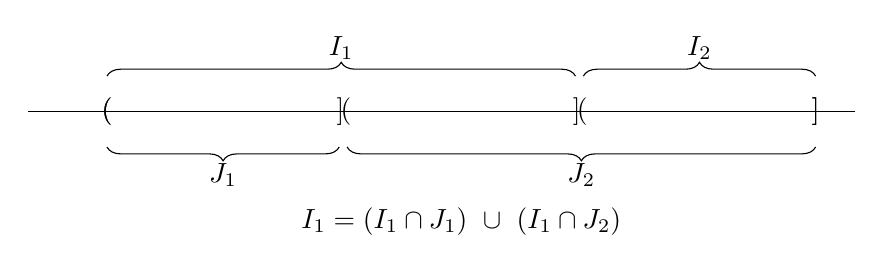
\begin{tikzpicture}[x=1cm,y=1cm]
                    \def\L{0.5}
                    \def\a{1.5}
                    \def\c{4.5}
                    \def\d{7.5}
                    \def\b{10.5}
                    \draw (\L,0) -- (\b+0.5,0);

                    % braces with small separation
                    \draw[decorate,decoration={brace,amplitude=5pt}]
                        (\a,0.45) -- ({\d-0.05},0.45) node[midway,yshift=10pt] {$I_1$};
                    \draw[decorate,decoration={brace,amplitude=5pt}]
                        ({\d+0.05},0.45) -- (\b,0.45) node[midway,yshift=10pt] {$I_2$};
                    \draw[decorate,decoration={brace,mirror,amplitude=5pt}]
                        (\a,-0.45) -- ({\c-0.05},-0.45) node[midway,yshift=-10pt] {$J_1$};
                    \draw[decorate,decoration={brace,mirror,amplitude=5pt}]
                        ({\c+0.05},-0.45) -- (\b,-0.45) node[midway,yshift=-10pt] {$J_2$};

                    % interval marks
                    \node at (\a,0) {$($};
                    \node[xshift=-1pt] at (\d,0) {$]$};
                    \node[xshift= 1pt] at (\d,0) {$($};
                    \node at (\b,0) {$]$};

                    \node at (\a,0) {$($};
                    \node[xshift= -1pt] at (\c,0) {$]$};
                    \node[xshift= 1pt] at (\c,0) {$($};
                    \node at (\b,0) {$]$};

                    % equation below
                    \node at ({(\a+\b)/2},-1.4)
                        {$I_1 = (I_1 \cap J_1)\ \cup\ (I_1 \cap J_2)$};
                \end{tikzpicture}
                } % end resizebox
                \caption{Illustration of interval intersections between $I_1$, $I_2$, and $J_1$, $J_2$.}
                \label{fig:interval_union}
            \end{figure}
            (\textit{See Figure 2.1 as a motivating example}). Apply the special case inside each $I_i$ and $J_j$:
                \begin{equation*}
                \begin{split}
                    \mu_0(I_i) = \sum_{j = 1}^n \mu_0 (I_i \cap J_j), \h9\h4 \mu_0(J_j) = \sum_{i = 1}^n \mu_0 (I_i \cap J_j).
                \end{split}
                \end{equation*}
            Summing each equation and rearranging gives $\sum_{i = 1}^n \mu_0(I_i) = \sum_{i,j}\mu_0 (I_i \cap J_j) = \sum_{j = 1}^n \mu_0(J_j)$. Thus $\mu_0$ is well-defined.

            We only need to show that $\mu_0$ satisfies countable additivity. Let $\{A_j\}_{j = 1}^\infty \subset \cA$ be a family of disjoint sets, where $\bigcup_{j = 1}^\infty A_j \in \cA$. Since everything in $\cA$ is a finite disjoint union of $h$-intervals, we can write:
                \begin{equation*}
                \begin{split}
                    \bigcup_{j = 1}^\infty A_j = \bigcup_{n = 1}^N I_n, \h9\h4 A_j = \bigcup_{i = 1}^{N_j}I_{i,j}.
                \end{split}
                \end{equation*}
            But observe that:
                \begin{equation*}
                \begin{split}
                    I_n 
                    & = I_n \cap  \left(\bigcup_{j = 1}^\infty A_j \right)\\
                    & = \bigcup_{j = 1}^\infty (I_n \cap A_j) \\
                    & = \bigcup_{j = 1}^\infty \left( I_n \cap \left( \bigcup_{i = 1}^{N_j}I_{i,j}\right) \right) \\
                    & = \bigcup_{j = 1}^\infty \bigcup_{i = 1}^{N_j} (I_n \cap I_{i,j}).
                \end{split}
                \end{equation*}
            It is enough to assume that if an $h$-interval $I$ is a countable disjoint union of $h$-intervals $\{I_j\}_{j = 1}^\infty$, then $\mu_0(I) = \sum_{j = 1}^\infty \mu_0(I_j)$. Let $I = (a,b]$ and $I_j = (a_j,b_j]$. One direction of the equality can be seen as folllows:
                \begin{equation*}
                \begin{split}
                    \mu_0(I) 
                    & = \mu_0\left(\bigcup_{j = 1}^n I_j\right) + \mu_0\left(I \setminus \bigcup_{j = 1}^n I_j\right) \\
                    & \geq \mu_0 \left( \bigcup_{j = 1}^n I_j \right) \\
                    & = \sum_{j = 1}^n \mu_0(I_j).
                \end{split}
                \end{equation*}
            Taking $n \rightarrow \infty$ gives $\mu_0(I) \geq \sum_{j = 1}^\infty \mu_0(I_j)$. Conversely, let $\epsilon > 0$. By the right-continuity of $F$, choose $\delta > 0$ such that $F(a + \delta) - F(a) < \epsilon$. Similarly, choose $\delta_j > 0$ such that $F(b_j + \delta_j) - F(b_j) < \frac{\epsilon}{2^j}$. Then the compact set $[a+\delta,b]$ is covered by the open intervals $\{(a_j,b_j + \delta_j\}_{j = 1}^\infty $, so there exists a finite subcover $\{ (a_j,b_j]\}_{j = 1}^N$. Without loss of generality, let $a_1 < a_2 < ... < a_N$. By construction $b_j + \delta_j \in (a_{j + 1}, b_{j+1} + \delta_{j+1})$. We then get:
                \begin{equation*}
                \begin{split}
                    \mu_0(I)
                    & = F(b) - F(a) \\
                    & \leq F(b) - F(a+\delta) + \epsilon \\
                    & = F(b_N + \delta_N) - F(a_N) + \sum_{j = 1}^{N-1} \bigl(F(a_{j+1}) - F(a_j)\bigr) + \epsilon \\
                    & \leq F(b_N + \delta_N) - F(a_N) + \sum_{j = 1}^{N-1} \bigl(F(b_j + \delta_j) - F(a_j)\bigr) + \epsilon \\
                    & = \sum_{j = 1}^{N} \bigl(F(b_j + \delta_j) - F(a_j)\bigr) + \epsilon \\
                    & < \sum_{j = 1}^{N} \bigl(F(b_j) + \frac{\epsilon}{2^j} - F(a_j)\bigr) + \epsilon \\
                    & \leq \sum_{j = 1}^N \bigl(F(b_j) - F(a_j)\bigr) + 2 \epsilon \\
                    & = \sum_{j = 1}^N \mu_0(I_j) + 2 \epsilon \\
                \end{split}
                \end{equation*}
            Taking $\epsilon \rightarrow 0$ finally shows that $\mu_0$ is countable additive over disjoint unions of $h$-intervals. Thus, $\mu_0$ is a well-defined premeasure defined on $\cA$, the algebra of countable disjoint unions of $h$-intervals.
        \end{proof}

    Having finally constructed the premeasure $(\bfR, \cA, \mu_0)$, we can now apply \nameref{thm:premeasure}.

    \begin{theorem}
        Let $F$ be a distribution function. There is a unique Borel measure $\mu_F$ on $\bfR$ such that $\mu_F((a,b]) = F(b) - F(a)$. If $G$ is another such function, then $\mu_F = \mu_G$ if and only if $F-G$ is constant. Conversely, if $\mu$ is a Borel measure on $\bfR$ that is finite on all bounded Borel sets, define:
            \begin{equation*}
            \begin{split}
                F(x) =
                \begin{cases}
                    \mu ( (0,x]), & x > 0, \\
                    0, & x = 0, \\
                    \mu ( -(x,0]), & x < 0, \\
                \end{cases}
            \end{split}
            \end{equation*}
        Then $F$ is a distribution, and $\mu = \mu_F$.
    \end{theorem}
        \begin{proof}
            Proposition~\ref{prop:premeasures-well-defined} showed that each $F$ induces a premeasure on $\cA$, the collection of countable disjoint unions of $h$-intervals. It is clear that $F$ and $G$ induce the same premeasure if $F-G$ is constant, and that these premeasures are $\sigma$-finite. The assertion that there is a \textit{unique} Borel measure comes from \nameref{thm:premeasure}. Given the outer measure $\mu^\ast$, induced by the premeasure on countable disjoint unions of $h$-intervals, define $\mu_F := \restr{\mu^\ast}{\fM(\cA)} = \restr{\mu^\ast}{\cB_\bfR}$. The converse direction follows from the monotonicity of $\mu$.
        \end{proof}

    There are many levels to this application of Theorem~\ref{thm:caratheodory}, Theorem~\ref{thm:premeasure}, and Proposition~\ref{prop:premeasures-well-defined}. Different restrictions of the outer-measure space $(X,\cP(X),\mu^\ast)$ give different $\sigma$-algebra to work in. We have the chain of $\sigma$-algebras:
        \begin{equation*}
        \begin{split}
            \cA \subset \cB_\bfR \subsetneq \cM^\ast \subset \cP(X),
        \end{split}
        \end{equation*}
    Where $\mu_F := \restr{\mu^\ast}{\fM(\cA)} = \restr{\mu^\ast}{\cB_\bfR}$ is the measure on $\cB_\bfR$, and $\restr{\mu^\ast}{\cM^\ast}$ is the \textit{complete} measure on $\cM^\ast$, the set of all $\mu^\ast$-measurable sets. One can rigorously show that the domain of $\restr{\mu^\ast}{\cM^\ast}$ is strictly larger than the domain of $\restr{\mu^\ast}{\cB_\bfR}$.

    \begin{definition}
        Let $\mu_0$ be a premeasure on $\cA$ (the algebra of countable disjoint unions of $h$-intervals) and $F$ a distribution function on $\mu_0$. The restriction of the $(X,\cA,\mu_0)$ induced outer measure onto all measurable sets is called the \textit{Lebesgue-Stieltjes measure associated to F}.
    \end{definition}

    For the remainder of this section, let $\mu$ denote the Lebesgue-Stieltjes measure on $\bfR$ associated to the distribution function $F$, and $\cM_\mu$ the domain of $\mu$.

    \begin{theorem}
        If $E \in \cM_\mu$, then:
            \begin{equation*}
            \begin{split}
                \mu(E) 
                &= \inf\{\mu(U) \mid U \supset E \text{ and }U \text{ is open }\} \\
                & = \sup\{\mu(K) \mid K \subset E \text{ and }K \text{ is compact }\} \\
            \end{split}
            \end{equation*}
    \end{theorem}
        {\color{red} \begin{proof}
        
        \end{proof}}

    \newpage

    \begin{theorem}***
        Let $F:\bfR \rightarrow \bfR$ be an increasing and right-continuous function. There exists a unique measure $\mu_F$ on $\cB_\bfR$ such that $\mu((a,b]) = F(b) - F(a)$. for all $a,b$. If $G$ is another such function, we have $\mu_F = \mu_G$ if and only if $F-G$ is constant. Conversely, if $\mu$ is a measure on $\cB_\bfR$ that is finite on all bounded Borel sets adding we define:
            \begin{equation*}
            \begin{split}
                F(x) = \begin{cases}
                    \mu((0,x]), & x > 0 \\
                    0, & x = 0 \\
                    -\mu((x,0]), & x < 0 ,\\
                \end{cases}
            \end{split}
            \end{equation*}
        then $F$ is increasing, right continuous, and $\mu = \mu_F$.
    \end{theorem}
        {\color{red} \begin{proof}
            10/8/25
        \end{proof}}

    Note that we have the following chain of inclusions:
        \begin{equation*}
        \begin{split}
            \cA \subset \cB_\bfR \subsetneq \cM_\mu \subset \cP(\bfR)
        \end{split}
        \end{equation*}
    This theorem gave us a measure $\mu^\ast$ on $\cM_\mu$, but we only really every cared about measures on $\cB_\bfR$ since they are generated by nice sets. We got a good bang for our buck. {\color{red} Are we talking about sets on $\cB_\bfR$ or sets on $\cM_\mu$?} Okay so basically the book is saying that $\restr{\mu^\ast}{\fM(\cA)} := \mu_F$... BUT.... we have the complete measure $\mu^\ast := \overline{\mu_F}$ on $\cM^\ast:= \cM_\mu$... Basically we are talking about properties that hold on $\cM^\ast := \cM_\mu$ (caratheodoyrys extension theorem gave us this $\cM^\ast$,... ) Ignore what I just said and look at this table:
        \begin{equation*}
        \begin{split}
            \cA &\leftrightarrow \mu_0 \\
            \cB_\bfR &\leftrightarrow \restr{\mu^\ast}{\fM(\cA)} \\
            \cM_\mu &\leftrightarrow \restr{\mu^\ast}{\cM_\mu} \\
            \cP(\bfR) &\leftrightarrow \mu^\ast
        \end{split}
        \end{equation*}
    We're gonna be proving properties on $\cM_\mu$

    \begin{definition}
        A measure satisfying the property from Proposition~\ref{}
    \end{definition}

    For the remainder of this section we will fix a complete Lebesgue-Stieltjes measure $\mu$ on $\bfR$ associated to the increasing, right continuous function $F$. We denote by $\cM_\mu$ the domain of $\mu$. {\color{red} Also, the notation in Folland is horrible}


    \begin{theorem}
        Let $E \subset \cM_\mu$.
        \begin{enumerate}[label = (\arabic*),itemsep=1pt,topsep=3pt]
            \item $\mu(E) = \inf \{\mu(U) \mid U \supset E, \h1 U \text{ open }\}$.
            \item $\mu(E) = \sup\{\mu(K) \mid K \subset E, \h1 K \text{ compact }\}$.
        \end{enumerate}
    \end{theorem}
        {\color{red} \begin{proof}
        
        \end{proof}}

{\color{blue} \section*{Da Homework:}
\begin{exercise}
Let $\cA \subset \cP(X)$ be an algebra, $\cA_\sigma$ the collection of countable unions of sets in $\cA$, and $\cA_{\sigma\delta}$ the collection of countable intersections of sets in $\cA_\sigma$. Let $\mu_0$ be a premeasure on $\cA$ and $\mu^\ast$ the induced outer measure.
    \begin{enumerate}[label = (\alph*),itemsep=1pt,topsep=3pt]
        \item For any $E \subset X$ and $\epsilon > 0$ there exists $A \in \cA_\sigma$ with $E \subset A$ and $\mu^\ast(A) \leq \mu^\ast(E) + \epsilon$.
        \item If $\mu^\ast(E) < \infty$, then $E$ is $\mu^\ast$-measurable if and only if there exists $B \in \cA_{\sigma\delta}$ with $E \subset B$ and $\mu^\ast(B \setminus E) = 0$.
        \item If $\mu_0$ is $\sigma$-finite, the restriction $\mu^\ast(E) < \infty$ in (b) is superfluous.
    \end{enumerate}
\end{exercise}
    \begin{proof}
        (a) Let $E \subset X$ and $\epsilon > 0$. By the defintion of $\mu^\ast(E)$, we can find $\{A_j\}_{j = 1}^\infty \subset \cA$ such that $\bigcup_{j = 1}^\infty A_j \supset E$ and: 
            \begin{equation*}
            \begin{split}
                \mu^\ast(E) + \epsilon 
                & \geq \sum_{j = 1}^\infty \mu_0(A_j) \h9\h9\h8\text{\tiny Property of infimums}\\ 
                & = \sum_{j = 1}^\infty \mu^\ast (A_j) \h9\h9\h9 \text{\tiny Because $\restr{\mu^\ast}{\cA} = \mu_0$}\\
                & \geq \mu^\ast \left( \bigcup_{j = 1}^\infty A_j \right). \h9\h9\h1\text{\tiny Outer measures are subadditive}
            \end{split}
            \end{equation*}

        (b) ($\Rightarrow$) Suppose $E$ is $\mu^\ast$-measurable. By (a), for every $n \in \bfN$, there exists $A_n \in \cA_\sigma$ such that $E \subset A_n$ and $\mu^\ast (A_n) \leq \mu^\ast (E) + \frac{1}{n}$. Since $\mu^\ast(E) < \infty$, we have $\mu^\ast(A_n) - \mu^\ast(E) \leq \frac{1}{n}$. Define $B = \bigcap_{n = 1}^\infty A_n \in \cA_{\sigma\delta}$. Then for all $n \in \bfN$:
            \begin{equation*}
            \begin{split}
                \mu^\ast(B \setminus E)
                & = \mu^\ast(B \cap E^c) \\
                & \leq \mu^\ast (A_n \cap E^c) \h9\h9\h9\h9
                \h9\h9\text{\tiny Monotonicity \& $B \subset A_n$ $\forall n$}\\
                & = \mu^\ast(A_n) - \mu^\ast(A_n \cap E) \h9\h9\text{\tiny Since $E$ is $\mu^\ast$-measurable} \\
                & = \mu^\ast(A_n) - \mu^\ast(E) \h9\h9\h9\h9\h8 \text{\tiny Since $E \subset A_n$}\\
                & \leq \frac{1}{n} 
            \end{split}
            \end{equation*}
        Hence $\mu^\ast(B \setminus E) = 0$. ($\Leftarrow$) Now let $B \in \cA_{\sigma\delta}$ such that $E \subset B$ and $\mu^\ast(B \setminus E) = 0$. Apply part (a) to the set $B \setminus E$. For each $n \in \bfN$, there exists $A_n \in \cA_\sigma$ such that $B\setminus E \subset A_n$ and $\mu^\ast(A_n) \leq \mu^\ast (B \setminus E) + \frac{1}{n} = \frac{1}{n}$. Since $A_\sigma \subset \fM(\cA) \subset \cM^\ast$, and since $\cM^\ast$ is a $\sigma$-algebra, the set $\bigcap_{n = 1}^\infty A_n$ is measurable. Since $B \setminus E \subset A_n$ for every $n \in \bfN$, we have $B \setminus E \subset \bigcap_{n = 1}^\infty A_n$. Since $\bigcap_{n = 1}^\infty A_n \subset A_n$, for every $n \in \bfN$ we have $\mu^\ast \left( \bigcap_{n = 1}^\infty A_n \right) \leq \mu^\ast(A_n) \leq \frac{1}{n}$. Hence $\mu^\ast \left( \bigcap_{n = 1}^\infty A_n \right) = 0$. Since $(X, \cM^\ast , \restr{\mu^\ast}{\cM^\ast})$ is a complete measure space, and since $\bigcap_{n= 1}^\infty A_n$ is a null-set, every subset of $\bigcap_{n= 1}^\infty A_n$ is measurable. In particular, $B \setminus E$ is measurable. Moreover, $B \in \cA_{\sigma\delta} \subset \cM^\ast$, hence $B$ is also measurable. We can write $E = B \setminus (B \setminus E) = B \cap (B \setminus E)^c$. Note that $B \in \cM^\ast$, and $(B \setminus E)^c \in \cM^\ast$ since $B \setminus E \in \cM^\ast$ and since $\cM^\ast$ is closed under intersections (it is a $\sigma$-algebra), hence $E \in \cM^\ast$ meaning that it is measurable.

        (c) We did not use the restriction $\mu^\ast (E) < \infty$ in the ($\Leftarrow$) direction, hence we only need to prove ($\Rightarrow$) for when $\mu_0$ is $\sigma$-finite. Let $X = \bigcup_{j = 1}^\infty X_j$. Then $\mu_0(X_i) < \infty$. Define $E_n = E \cap \left( \bigcup_{j = 1}^n X_j \right)$. Then $\bigcup_{n = 1}^\infty E_n = E$. \nl
        
        \noindent For every $n \in \bfN$, apply part (a) to $E_n$. \nl
        
        \noindent There exists $C_n \in \cA_\delta$ such that $E_n \subset C_n$ and $\mu^\ast(C_n) \leq \mu^\ast(E_n) + \frac{1}{n}$. Define $C = \bigcap_{n = 1}^\infty C_n$. Then $\mu^\ast(C) \leq \mu^\ast(C_n) \leq \mu^\ast(E_n) + \frac{1}{n}$. Rearranging gives $\mu^\ast(C) - \mu^\ast(E_n) \leq \frac{1}{n}$. But since $\mu^\ast(E_n) \leq \mu^\ast(E)$, we have $\mu^\ast(C) - \mu^\ast(E) \leq \mu^\ast(C) - \mu^\ast(E_n) \leq \frac{1}{n}$. Since this holds true for all $n \in \bfN$, we have $\mu^\ast(C \setminus E) = 0$.
    \end{proof}
%%%%%%%%%%%%%%%%%%%%%%%%%%%%%%%%%%%%%%%%%%%%%%%%%%
\begin{exercise}
    Let $\mu^\ast$ be an outer measure on $X$ induced by the finite premeasure $\mu_0$. If $E \subset X$, define the \textit{inner measure} of $E$ to be $\mu_\ast(E) = \mu_0(X) - \mu^\ast(E^c)$. Show $E$ is $\mu^\ast$-measurable if and only if $\mu^\ast(E) = \mu_\ast(E)$.
\end{exercise}
    \begin{proof}
        ($\Rightarrow$) Suppose $E$ is $\mu^\ast$-measurable. Then $E^c$ is also $\mu^\ast$-measurable since $\cM^\ast$ is a $\sigma$-algebra. We can write:
            \begin{equation*}
            \begin{split}
                \mu^\ast (X) = \mu^\ast(E) + \mu^\ast(E^c).
            \end{split}
            \end{equation*}
        Since $X\in \cA$ and $\mu_0 = \restr{\mu^\ast}{\cA}$, we have:
            \begin{equation*}
            \begin{split}
                \mu_0(X) = \mu^\ast(E) + \mu^\ast(E^c).
            \end{split}
            \end{equation*}
        Subtracting both sides by $\mu^\ast(E^C)$ gives $\mu_\ast(E) = \mu^\ast(E)$. 

        ($\Leftarrow$) Now suppose $\mu^\ast(E) = \mu_0(X) - \mu^\ast(E^c)$. Again, since $X\in \cA$ and $\mu_0 = \restr{\mu^\ast}{\cA}$, we have:
            \begin{equation*}
            \begin{split}
                \mu^\ast(E) + \mu^\ast(E^c) = \mu^\ast(X) = \mu_0(X) < \infty
            \end{split}
            \end{equation*}
        For each $n \in \bfN$, Apply Exercise 1, part (a) to $E$. Then there exists $A_n \in \cA_\sigma$ such that $E \subset A_n$ and $\mu^\ast(A_n) \leq \mu^\ast(E) + \frac{1}{n}$. Define $B := \bigcap_{n = 1}^\infty A_n$. Note that $B$ is measurable since $B \in \cA_{\sigma\delta} \subset \cM^\ast$. Moreover since $E \subset A_n$ for all $n \in \bfN$, we have $E \subset B$. Together:
            \begin{equation*}
            \begin{split}
                \mu^\ast(E) \leq \mu^\ast(B) \leq \mu^\ast(A_n) \leq \mu^\ast(E) + \frac{1}{n}.
            \end{split}
            \end{equation*}
        Since this holds true for all $n \in \bfN$, it must be that $\mu^\ast(E) = \mu^\ast(B)$. Quickly note:
            \begin{equation*}
            \begin{split}
                \mu^\ast(B) + \mu^\ast(B^c) 
                & = \mu^\ast(X) \\
                & = \mu^\ast(E) + \mu^\ast(E^c).
            \end{split}
            \end{equation*}
        Since $\mu^\ast(B) = \mu^\ast(E) < \infty$, we have $\mu^\ast(E^c) = \mu^\ast(B^c)$. Now by the measurability of $B$:
            \begin{equation*}
            \begin{split}
                \mu^\ast (E) + \mu^\ast(E^c) 
                & = \mu^\ast(E) + \mu^\ast(E^c \cap B) + \mu^\ast(E^c \cap B^c) \\
                & = \mu^\ast(E) + \mu^\ast(E^c \cap B) + \mu^\ast(B^c) \\
                & = \mu^\ast(E) + \mu^\ast(E^c \cap B) + \mu^\ast(E^c) \\
            \end{split}
            \end{equation*}
        Hence $\mu^\ast(E^c \cap B) = \mu^\ast(B \setminus E) = 0$. By Exercise 1, part (b), $E$ is $\mu^\ast$-measurable.
    \end{proof}}



    



    


    


    
